\section{Physics of  Neutron Stars (NS)}


\begin{frame}
\begin{center}
 
	{\bf  ANALYTIC EQUATION OF STATE}
\end{center}

\end{frame}

\subsection*{Neutron Stars Overview}
\begin{frame}
\frametitle{Neutron Stars Overview}  
\begin{columns}[c]
\begin{column}{0.65\textwidth} 
\begin{enumerate}
\scriptsize{
 \item Objects with {\bf most extreme densities ($\rho$)}  and {\bf strongest magnetic field (B)}.
 
 \quad
 
 \item  {\bf Energetically favorable} for protons and electrons to form {\bf free neutrons}, generating the {\bf degeneracy pressure}.\\ {\tiny (but core exhibits collective behavior of particles)}
% Free neutrons normally $\beta$ decay in $\sim 15$ minutes, but at sufficient depths in the NS the decay reaction is suppressed as the Fermi energy becomes too high to be populated by the electrons which would be created in the decay. 
 
 \quad
  
 
\item Observations of NSs constrain the physics of their {\bf interiors}:
\begin{itemize}\scriptsize{
 \item {\bf low temperatures},
 \item $\rho \gg$ {\bf  nuclear saturation density}. \\{\tiny ($\rho_s \sim 2.7 \times 10^{14}$ g cm$^{-3})$}}
\end{itemize}

  \quad
  
 
 \item {\bf Photons emitted} from the NS {\bf surface} are direct probes of their {\bf structure, composition, and magnetic field}.
 
 \quad
 
 \item Determining the {\bf EoS} of this {\bf cold ultradense matter} is a {\bf challenge} of high-energy and nuclear astrophysics!

 }
 
\end{enumerate}
\end{column}
\begin{column}{0.5\textwidth}    
 \center{\tiny QCD phase diagram:\\
 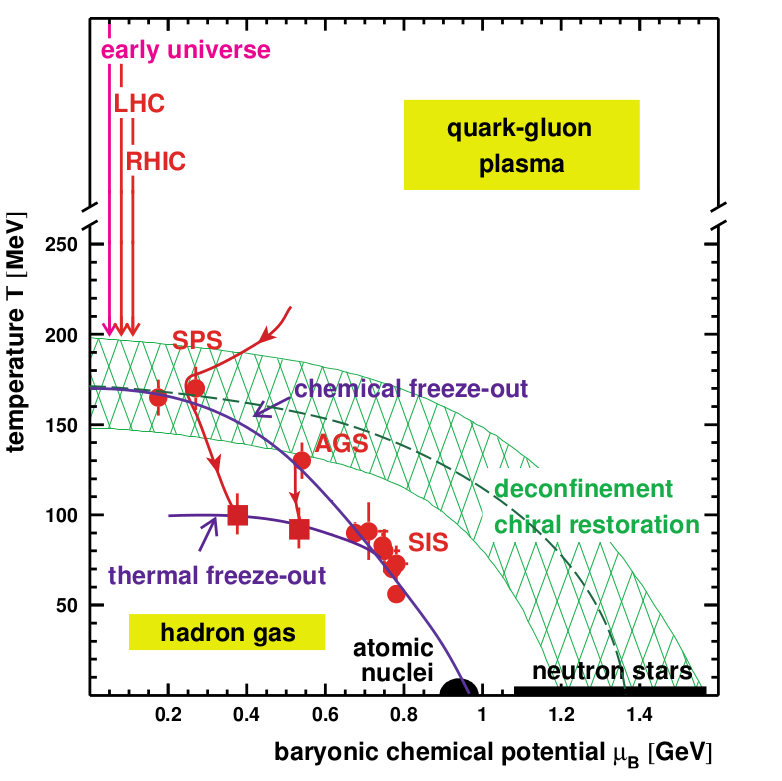
\includegraphics[scale=0.2]{figs/phasetran.png}\\
 High-density/low T region is inaccessible to terrestrial \\experiments (Paerels et al, 2009).}
\end{column}
\end{columns} 
\end{frame}






%%%%%%%%%%%%%%%%%%%%%%%%%%%%%%%%%%%%%%%%%%%%%%%%%%%%%%%%%%%%%%%%%%%%%%%%%%%%%%%%%%%

\subsection*{Neutron Star Radii and Compactness}
\begin{frame}
\frametitle{Neutron Star Radii and Compactness}

\begin{columns}[c]
\begin{column}{0.55\textwidth}

\begin{itemize}
\scriptsize{
\item  {\bf NS EoS} is hard to be obtained from first principles.

\quad
 
 \item Matter that can only be probed through astrophysical observations of {\bf mass} and {\bf radius} with {\bf sufficient precision}!  \\{\tiny (Lattimer $\&$ Prakash , 2007)}
 
 \quad
 
\item Unique map between microscopic {\bf (P-$\rho$)} and macroscopic {\bf(M-R)}.


\quad

\item For instance, $M_{NS}=1.4 M_{\odot}$ gives determination of pressure at $2 \rho_s$.\\ {\tiny (Lattimer $\&$ Prakash , 2011)}
}


\end{itemize}
\end{column}

\begin{column}{0.6\textwidth}
 \center{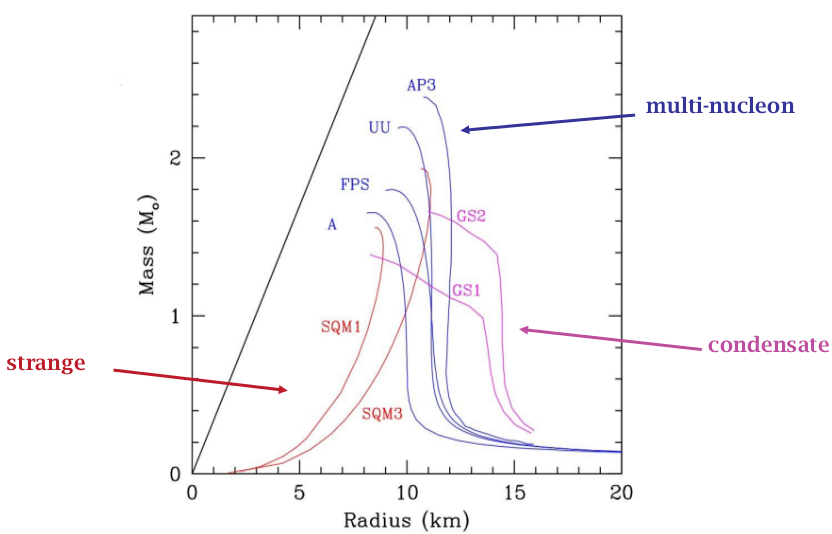
\includegraphics[scale=0.2]{figs/oz.png}}\\
	{\tiny {\bf Mass-radius relations for a selection of NS EoS}: \\{\bf APR} (Akmal et al., 1998), {\bf MS} (M\"uller \& Serot, 1996), {\bf GS} (Glendenning \& Schaffner-Bielich, 1999), {\bf  ABPR }(Alford et al., 2005),  {\bf BBB} (Brueckner-Hartree-Fock model), {\bf SQM }(Prakash et al., 1995).}
 \end{column}
 \end{columns}
\end{frame}



%%%%%%%%%%%%%%%%%%%%%%%%%%%%%%%%%%%%%%%%%%%%%%%%%%%%%%%%%%%%%%%%%%%%%%%%%%%%%%%%%%%


\subsection*{How to Obtain R and M?}
\begin{frame}
\frametitle{Some Initial Quantities to infer (M,R)}

\begin{columns}[c]
\begin{column}{0.6\textwidth} 

\begin{enumerate}\scriptsize{
\item Observational appearance of NS affected by {\bf redshift and lensing effects}.

\quad



\item The {\bf redshift} is
$$1+z = |g_{tt}|^{-1/2} = \Big(1 - \frac{2GM}{Rc^2} \Big)^{-1/2}.$$



\item The apparent radius at some distance $D$ is then
$$R_{\infty} = R \Big( 1 - \frac{2GM}{Rc^2}\Big)^{-1/2}.$$



%\item (M-R) relation are given by $R = R_{\infty} (1 + z) -1 ,$
%$M = R_{\infty} c^2 (1 + z)-1= [1 - (1 + z)^{-2} ]/2G.$

\item {\bf Lensing} from a {\bf strong gravitational field} gives an area which  appears to be large by 
$$\frac{S_{\infty}}{4\pi R^2} = (1+z)^2.$$


}
\seti
\end{enumerate}
\end{column}
\begin{column}{0.6\textwidth} 
\begin{enumerate}\scriptsize{
\conti


%\item The {\bf  Eddington luminosity at infinity } is:
%$L_{E,\infty} = \frac{8\pi m_pc}{(1+X)\sigma_T} \Big (1 - \frac{2GM}{Rc^2} \Big)^{1/2}.$

\item The {\bf  total flux } observed at distance $D$ is 
$$F_{\infty} = \sigma_B T^4_{eff,\infty} \Big ( \frac{R}{D} \Big)^2 (1+z)^2.$$


\item  Uncertainties given by:
\begin{itemize}\scriptsize{
 \item {\bf distance} ($R_{\infty} \propto D$),
 \item  {\bf interstellar H absorption},
 \item and {\bf atmospheric composition}. }
\end{itemize}

\quad

\item {\bf Best probes}: 
\begin{itemize}\scriptsize{
 \item nearby isolated NS (parallax measurable),
 \item and X-ray binaries in globular clusters.
}\end{itemize}

}
\end{enumerate}
 \end{column}
 \end{columns}
\end{frame}




%%%%%%%%%%%%%%%%%%%%%%%%%%%%%%%%%%%%%%%%%%%%%%%%%%%%%%%%%%%%%%%%%%%%%%%%%%%%%%%%%%%

\subsection*{Energy Sources in Neutron Stars}

\begin{frame}
\frametitle{Energy Sources in Neutron Stars:}  
\begin{enumerate}
 \item Radiation of Residual Heat in Young NSs.
 
 \quad
 
 \item Re-radiation of deposition heat between accretion episodes.
 
 \quad
 
 \item Magnetic Field Decay.
 
 \quad

 \item Particle Bombardment onto Polar Caps.
 
  \quad
 
 \item {\bf Thermonuclear Bursts}.
 
\end{enumerate}
\end{frame}







%%%%%%%%%%%%%%%%%%%%%%%%%%%%%%%%%%%%%%%%%%%%%%%%%%%%%%%%555



\section{Physics of NS Surface Emission}





%%%%%%%%%%%%%%%%%%%%%%%%%%%%%%%%%%%%%%%%%%%%%%%%%%%%%%%%%%%%%%%%%%%%%%%%%%%%%%%%%%%


\begin{frame}
\begin{center}
 
	{\bf  OBSERVATIONAL ASTROPHYSICS} 
\end{center}

\end{frame}


\subsection*{Observing Neutron Stars and their Surfaces} 

\begin{frame}
\frametitle{Observing Neutron Stars and their Surfaces} 

\begin{columns}[c]
\begin{column}{0.55\textwidth} 
	{\bf \center We probe NSs from:}{\scriptsize
	 \begin{enumerate}
	     \item Dynamics of {\bf binary systems}.
	     \item Structure and energetics of {\bf radio pulse sources}.
	     \item {\bf Spectra and variability} of their high energy radiation.
	     \item {\bf Direct observations} of the {\bf  surface emission} (often hidden from view).
	     	    \end{enumerate}
}
\end{column}
\begin{column}{0.55\textwidth}    
{\bf \center We see evidences of NS surface emission from:}
\begin{itemize}\scriptsize{
		 \item {\bf Thermonuclear bursters from (LMXB)}.
		 \item {\bf Accreting sources during quiescence}. {\tiny
		 \item Isolated cooling NS (DINS), central compact objects (CCO).
		 \item Pulsating sources in radio (PSR).
		 \item Accretion powered pulsars (AMSP) and accreting millisecond X-ray pulsars (MSP), Soft gamma-ray repeaters(SGR), anomalous X-ray pulsars (AXP).}}
	  \end{itemize}
	  \end{column}
\end{columns}
 \center{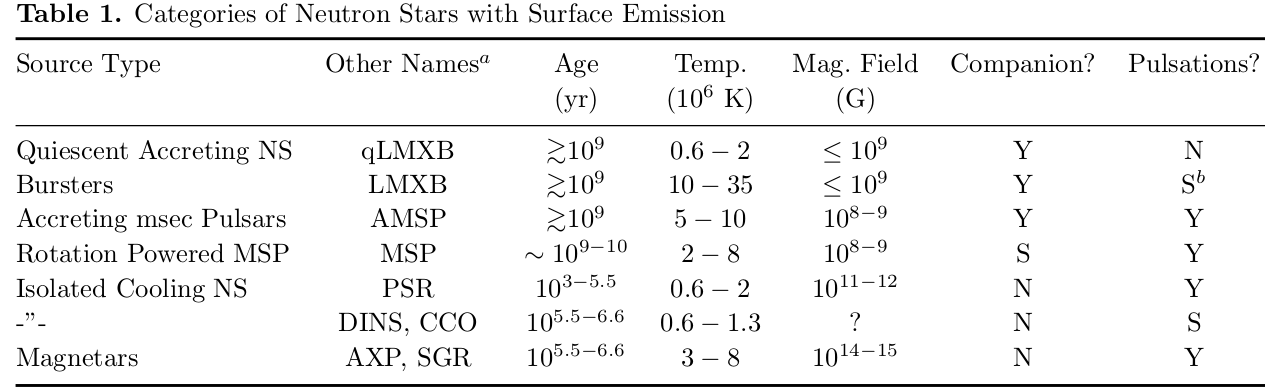
\includegraphics[scale=0.19]{figs/all.png}}

\end{frame}



%%%%%%%%%%%%%%%%%%%%%%%%%%%%%%%%%%%%%%%%%%%%%%%%%%%%%%%%%%%%%%%%%%%%%%%%%%%%%%%%%%%

\subsection*{Neutron Star Sources with Surface Emission}
\begin{frame}
\frametitle{Neutron Star Sources with Surface Emission}
\center{ {\bf Surface emission}  detected in many NS sources, with {\bf thermal spectra from optical to X-rays}: }

\begin{columns}[c]
\begin{column}{0.5\textwidth} 
 \scriptsize{
 \item {\bf Accreting NS in quiescence:} \\
 
 \quad
 
 \begin{itemize}\scriptsize{
 \item  Half of NS accreting from low-mass companion have X-ray transients.
 
 
 
 \quad
 
  \item {\bf X-rays transients} have several different accretion phases, varying flux level and spectral characteristics.
  
  \quad
  
  \item {\bf Outburst luminosity} $\sim 10^{36-38}$ erg s$^{-1}$, same order of their {\bf quiescent luminosity}.}
 \end{itemize}}

 


\end{column}
\begin{column}{0.65\textwidth}   

 \scriptsize{
 
\item {\bf Accreting Bursting NS (from LMXB):}\\

\quad

\begin{itemize}\scriptsize{

\item 100 of $\sim$ 150 exhibit thermonuclear bursts, with X-ray flux rising $\sim 10-100$ s.

\quad

 \item Due to {\bf unstable burning of He/H}, {\bf accreted} to the NS surface from companion.
 
 \quad
 
 \item  {\bf Evolution of the color temperature} in the burst: dip in the {\bf T} rises {\bf photospheric radius expansion} (PRE).
 

 
 }
 
 
\end{itemize}
} 

\end{column}
\end{columns}
\end{frame}


%%%%%%%%%%%%%%%%%%%%%%%%%%%%%%%%%%%%%%%%%%%%%%%%%%%%%%%%%%%%%%%%%%%%%%%%%%%%%%%%%%
\subsection*{Type I X-Ray Bursters and LMXBs  }
\begin{frame}
\frametitle{Type I X-Ray Bursters and LMXBs}

\begin{columns}[c]
\begin{column}{0.6\textwidth} 
\begin{enumerate}\scriptsize{
\item {\bf X-ray bursters} (XRB) are periodic and rapid increases in luminosity in the X-ray range.

\quad


\item XRB are composed of {\bf an accreting compact object} (NS) and a {\bf companion}, whose mass categorizes the system:
\begin{itemize}\scriptsize{
 \item High mass ($M > 10 M_{\odot}$), {\bf (HMXB)}.
 \item Low mass ($M < 1 M_{\odot}$), {\bf (LMXB)}.}
\end{itemize}

\quad

\item {\bf Low mass X-ray Bursters} (LMXB) are {\bf thermonuclear} XRB that can put constraints on the NS EoS.

\quad

 
 \item For instance, observations of {\bf NS during thermonuclear bursts} have led to the {\bf  first constraining measurements of NS radii}: \\9 km $<$ R $<$ 12 km. \\{\tiny (Lattimer $\&$ Brown, 2010)}


}
\end{enumerate}
\end{column}
\begin{column}{0.55\textwidth}

  \center{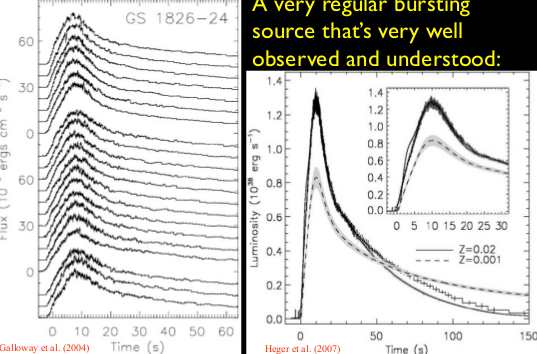
\includegraphics[scale=0.33]{figs/xx.png}}
\end{column}
\end{columns}
\end{frame}





%%%%%%%%%%%%%%%%%%%%%%%%%%%%%%%%%%%%%%%%%%%%%%%%%%%%%%%%%%%%%%%%%%%%%%%%%%%%%%%%%


\subsection*{Photospheric Radius Expansion (PRE) Bursts}
\begin{frame}
\frametitle{Photospheric Radius Expansion (PRE)}

\begin{columns}[c]
\begin{column}{0.55\textwidth} 

\begin{enumerate}
\scriptsize{
 \item  NS Observations are from the outermost layer of surface, the {\bf photosphere}, in radioactive equilibrium given by a flux 
$F=\sigma_B T^4_{eff}.$
 
 \quad

\item {\bf PRE bursts} are a {\bf bright} subset of TB where  at the so-called {\bf touchdown point} (where the {\bf photosphere} returns to the NS radius), fluxes are close to $L_{Edd} = 4 \pi R^2 \sigma_T T^4_{eff}.$ on the surface.

\quad

\item  $F_{Edd}$ can be related to the {\bf normalization of the burst spectrum} (blackbody normalization, $K$),  which gives the  {\bf emitting area} (R):


$$F_{Edd} = F_{touchdown} = \frac{GMc}{\kappa D^2} \Big ( 1 - \frac{2GM}{Rc^2} \Big)^{1/2},$$
$$ A = \frac{R^2}{D^2f_c^4} \Big( 1 - \frac{2GM}{Rc^2} \Big )^{-1} = f_c  K^{1/4},$$
 $f_c$ the color correction factor.


 }
  \end{enumerate}
  
  

\end{column}
\begin{column}{0.7\textwidth}
\begin{center}
\scriptsize{
Debate about {\bf systematic errors} that must be taken\\ into account ({\bf where is the touchdown?}). }
\\{\tiny (Suleimanov et al. 2011a; Guver, Ozel $\&$ Psaltis 2011)} 

\quad

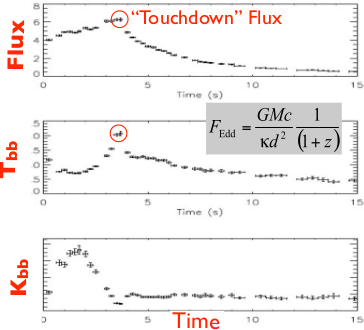
\includegraphics[scale=0.45]{figs/pree.png}
\end{center}

\quad 
  \end{column}
\end{columns}
   \end{frame}
   
   
 
 

\begin{frame}
\begin{center}
 
	{\bf  COMPUTATIONAL SIMULATIONS\\ AND FITTINGS} 
\end{center}

\end{frame}



\section{Modeling NS Atmospheres}

\subsection*{Parameters for Modeling Neutron Star Atmospheres}

\begin{frame}
\frametitle{Parameters for Modeling Neutron Star Atmospheres}

\begin{center}
 

	Detailed {\bf Models of NS atmospheres} shape the {\bf spectrum } and {\bf pattern of radiation} from {\bf crust and core}. 


\end{center}

	\begin{itemize}

	\item 
Assumptions:
\begin{enumerate}
 \item {\bf Plane-parallel} geometry.
 \item {\bf Radioactive equilibrium}.
 \item {\bf Hydrostatic equilibrium}.
\end{enumerate}
\quad

	 \item The {\bf four parameters} in the models are:
	   \begin{enumerate}
	    \item Magnetic field strengths;
	    \item Chemical Compositions (e.g. H fraction, $X$);
	    \item Temperature at surface, $T_{eff}$;
	    \item Gravitational acceleration at surface, $g$.
	   \end{enumerate}
	\end{itemize}	   
\end{frame}





%%%%%%%%%%%%%%%%%%%%%%%%%%%%%%%%%%%%%%%%%%%%%%%%%%%%%%%%%%%%%%%%%%%%%%%%%%%%%%%%%%%


\subsection*{Modeling the Spectrum of the  NS Surface Emission}



\begin{frame}
\frametitle{Some Results on Modeling and Fitting Spectra}
\begin{columns}[c]
\begin{column}{0.7\textwidth} 
\begin{enumerate}
\scriptsize{
\item Many different {\bf physical conditions}: {\tiny ( Suleimanov et al, 211)}
\begin{itemize}\scriptsize{
 \item 6 different {\bf chemical compositions} (pure H, pure He, solar mix, heavy elements).
 \item 3 values of {\bf surface gravities}.
 \item 20 values of {\bf luminosities} in units $l = L/L_{Edd}$.}
\end{itemize}

\quad
 
\item {\bf NS spectra} look like blackbody, but shifted to higher temperatures by the {\bf color coefficient factor}:
$$f_c = \frac{T_{BB}}{T_{eff}} = K^{-1/4}A $$

\item Fitting $f_cT_{eff}-l$ to the $K^{-1/4}-F_{\infty}$ on cooling LXRB  at some $D$, gives $$R_{\infty}=R(1+z)=R_{BB} f_c^2.$$ 

\quad

\item {\bf Others processes considered}: angular redistribution in scattering, electron conduction, {\bf Compton scattering}...
}
\end{enumerate}
\end{column}
\begin{column}{0.5\textwidth} 

 \center{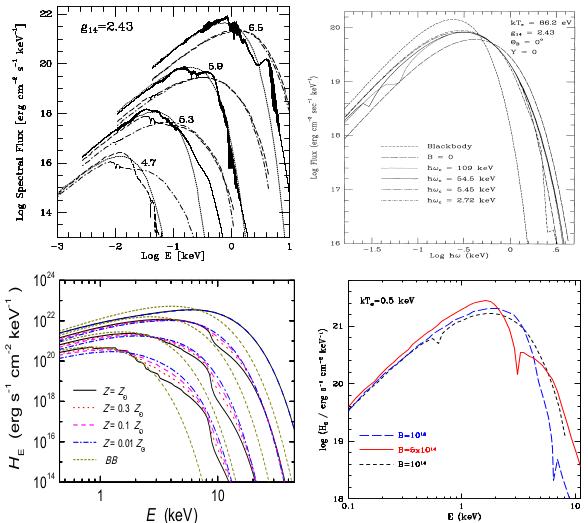
\includegraphics[scale=0.23]{figs/atms.png}}\\
 {\tiny Model spectra for four different types of NS, $H_E=4\pi H_E$: non-magnetic cool NS, cool with moderate B, hot bursting with mentalities, strong B with H.}

 \end{column}
 \end{columns}

\end{frame}


%%%%%%%%%%%%%%%%%%%%%%%%%%%%%%%%%%%%%%%%%%%%%%%%%%%%%%%%%%%%%%%%%%%%%%%
\subsection*{Some Results on Modeling and Fitting Spectra}

\begin{frame}
\frametitle{Results on Modeling and Fitting NS Spectra}
\begin{columns}[c]
\begin{column}{0.55\textwidth} 
 \center{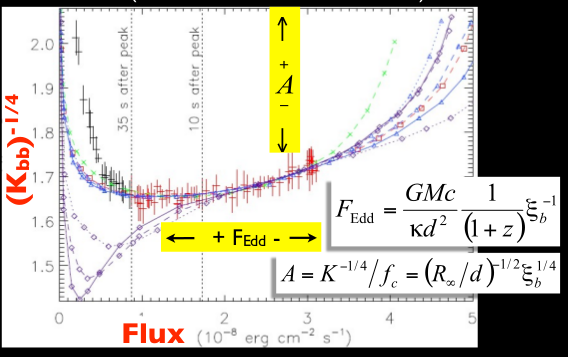
\includegraphics[scale=0.3]{figs/qqq.png}}\\
 {\tiny (Suleimanov et al, 2011)}\\
 

\end{column}
\begin{column}{0.55\textwidth} 
 \center{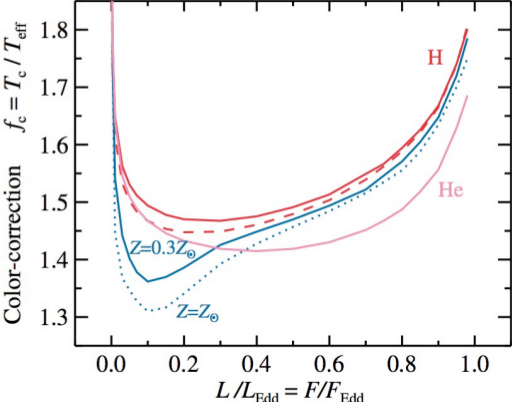
\includegraphics[scale=0.3]{figs/meu.png}}
  {\tiny (October/2012)}
 \end{column}
 \end{columns}
 
\end{frame}




\begin{frame}
\begin{center}
 
	{\bf  OUTLOOK}
\end{center}

\end{frame}

